
\resetcounters

\bibliographystyle{asp2010}

\markboth{Lorente, Farrell and Goodwin}{SAMI Automated Plug Plate Configuration}

\title{\ssindex{instruments!individual!SAMI}SAMI Automated Plug Plate Configuration}

\author{Nuria~P.~F.~Lorente, Tony~Farrell, and Michael~Goodwin
\affil{Australian Astronomical Observatory, PO Box 915,\\
North Ryde NSW 1670, Australia}
}

\aindex{Lorente, N. P. F.}
\aindex{Farrell, T.}
\aindex{Goodwin, M.}

\begin{abstract} The Sydney-AAO Multi-object Integral field spectrograph (\ssindex{instruments!individual!SAMI}SAMI) is a prototype wide-field system at the \ssindex{observatories!Earth-based!Anglo-AustralianTelescope}Anglo-Australian Telescope (AAT) which uses a plug-plate to mount its $13 \times 61$-core imaging fibre bundles (hexabundles) in the optical path at the telescope's prime focus. In this paper we describe the process of determining the positions of the plug-plate holes, where plates contain three or more stacked observation configurations. The process, which up until now has involved several separate processes and has required significant manual configuration and checking, is now being automated to increase efficiency and reduce error. This is carried out by means of a thin \ssindex{computer languages!Java}Java controller layer which drives the configuration cycle. This layer controls the user interface and the \ssindex{computer languages!C++}C++ algorithm layer where the plate configuration and optimisation is carried out. Additionally, through the \ssindex{applications!Aladin}Aladin\ooindex{Aladin, ascl:1112.019} display package, it provides visualisation and facilitates user verification of the resulting plates.
\end{abstract}

\section{Introduction}

The Sydney-AAO Multi-object Integral Field Spectrograph (\ssindex{instruments!individual!SAMI}SAMI) is a prototype wide-field system at the \ssindex{observatories!Earth-based!Anglo-AustralianTelescope}Anglo-Australian Telescope (AAT) deploying $13 \times 61$-core imaging fibre bundles (hexabundles) over a 1-degree field of view \citep{2012clb+}. The hexabundles, together with \ssindex{data!ancillary}ancillary sky and calibration fibres, are mounted on a plug plate located at the prime focus of the telescope. Each plate is a 24~cm diameter and 3~mm thick steel disc, pre-drilled with holes corresponding to the on-sky positions of targets for several distinct pointings. Typically this is 3 fields for science plates, and 8 fields in the case of plates used for the set-up and calibration of the instrument.
%
A science field consists of a guide-star located at the centre of the plate, a flux calibration star, 26 blank-sky positions and 12 science targets located in the 1-degree field-of-view. A calibration field contains either 2 visual alignment stars, used in the initial coarse plate rotation alignment process, or 13 stars used for distortion calculations and fine plate rotation alignment.

\section{Configuring the Plate}
The process of determining the positions of the science plate holes involves defining 3 stacked observing fields composed of a common guide-star hole at the centre of the plate, and choosing the flux star and science targets for each field taking into account separation constraints between targets in the same field and in the two other fields (simplistically, plug-holes should not overlap). The 26 blank-sky positions are allocated to each field with the additional constraint that only 26 sky holes are to be drilled in the plate, so the sky positions for each of the 3 fields must map to the same physical holes (see Figure~\ref{p048_FigStackedFields}). Configuration of the calibration plate holes is simpler, as there are no sky positions to find which are common to all fields, but star plates contain a greater number of stacked fields with one common guide-star hole: 4 visual alignment fields plus 4 fields for the astrometric distortion model and fine rotation alignment.

\begin{figure}[!t]
\centering
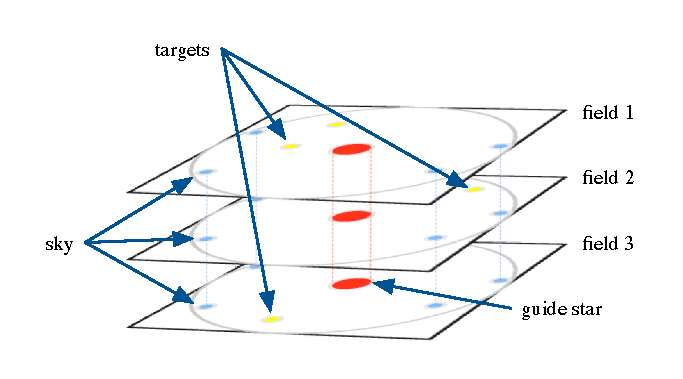
\includegraphics[width=0.7\linewidth]{part10/Lorente_P048/stackedFullPlate3dWithLabels.eps}
\caption {Representation of a science plate composed of three fields. The target positions are unique to a given field, whereas the sky positions are valid for each of the three field but use a single common hole on the plate.}
\label {p048_FigStackedFields}
\end{figure}

\noindent The steps involved in configuring a plate are as follows:
\begin{enumerate}
\item {\bf Field Creation:} From a target catalogue and a catalogue of suitable calibration and guide stars, a database of candidate observing fields is constructed, based on several positional constraints set by the physical limits imposed by the fibre connector assembly, the position of the guide camera and the need to physically place and remove connectors between one observation and the next. \newline 
- Separation between a target and the guide star: $7.6$\ arcmin $<$~separation $<0.5$~degrees\\
- Separation between two targets in the same field $> 3.8$\ arcmin

\item{\bf Field Stacking:} Taking into account inter-field exclusion rules, where the separation of two targets in different fields $>$3\ arcmin, multiple fields are stacked to form a single plate. Each field is taken from a different RA range, so that a night’s observation of 3 fields can be performed without the need to stop to change plates.

\item{\bf Sky Fibre Positioning:} A new method is being implemented for determining the position of the 26 sky fibres (Figure~\ref{p048_FigSkyPos}). First a grid is placed over the field with cell size = hole exclusion size / 2.  Any cells which fall within the exclusion zone of any star or target are then removed from the grid. The most isolated remaining cell is then located (i.e. the cell furthest from its nearest neighbour) and tested for suitability as a sky position. This involves checking that, in each of the 3 fields comprising the plate there are no sources above the magnitude limit within the sky fibre's field-of-view.  If the position is suitable, the grid cell is marked as full and the nearest-neighbour distances are recalculated.  This process is iterated until all 26 sky positions have been obtained.

\begin{figure}[ht]
\centering
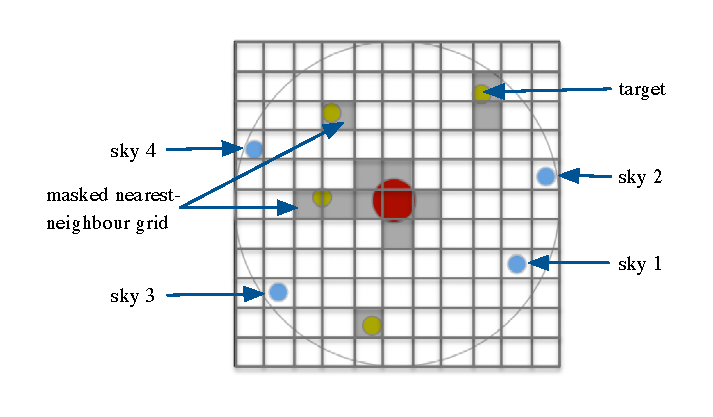
\includegraphics[width=0.7\linewidth]{part10/Lorente_P048/plateWithGrid3WithLabels.eps}
\caption {Finding suitable positions for sky fibres to ensure uniform coverage over the plate. This example shows the invalid (i.e. occupied) grid cells as gray and the order in which the sky positions have been determined (1 - 4).}
\label {p048_FigSkyPos}
\end{figure}

\item{\bf Transformation:} Once the plate positions are defined, instrument and sky compensation transforms are applied. These include the optical distortion model and the atmospheric differential refraction models, based on the expected time of observation of each field

\item{\bf Generation:} The configuration process creates two products: the first is a CSV file containing the hole positions for the plate. A final adjustment is made for the estimated dome temperature at observing time and ambient temperature at fabrication (when the holes are drilled) and these data are sent to the plate manufacturer. The second product is a set of observing files, which are used to drive the Telescope \ssindex{software!control system}Control System at observing time.

\item{\bf Verification and Visualisation:} Visualisation is done using the \ssindex{applications!Aladin}Aladin\ooindex{Aladin, ascl:1112.019} application \citep{2000bfb+}. The various components making up a plate --- the fields-of-view of the telescope, hexabundles, sky fibres and guide camera, the hole information and exclusion zones are separately layered onto an image of the field (Figure~\ref{p048_FigAladin}). This is done using the \ssindex{applications!Aladin}Aladin FoV mechanism, sending the relative positions from the centre of the field in a \ssindex{data formats!VOTable}VOTable format \citep{2011owd+}. The survey target positions are also plotted as a separate absolute position $(\alpha, \delta)$ layer. This facilitates  verification by eye of several items, including: 1) The target position is within the field-of-view of the fibre  hexabundle and that both of these coincide with the DSS galaxy; 2) The field-of-view of the sky fibres is empty, as expected; 3) The distribution of sky fibres is uniform across the plate; and 4) There are no bright stars or extended galaxies sufficiently close to a target position so as to pose a contamination risk.

\begin{figure}[ht]
\centering
\includegraphics[width=0.73\linewidth]{part10/Lorente_P048/aladinView.eps}
\caption{\ssindex{applications!Aladin}Aladin\ooindex{Aladin, ascl:1112.019} screenshot showing \ssindex{instruments!individual!SAMI}SAMI's $1^\circ$ field-of-view (white), guide camera (red), hexabundle (yellow)  and sky fibre (blue) positions, superimposed on a DSS image.}
\label{p048_FigAladin}
\end{figure}

\end{enumerate}


\section{Automation}
As part of a prototype project this configuration process has until now been a painstaking task involving the use of several software packages, scripts, stand-alone code and a lot of manual configuration and checking. As \ssindex{instruments!individual!SAMI}SAMI evolves from a technology demonstrator to a survey instrument with an expected observing catalogue of several thousand targets, this approach will no longer be feasible, for reasons of both efficiency and the increased likelihood of error.

Consequently, the process for configuring \ssindex{instruments!individual!SAMI}SAMI plates is now in the process of being automated. This consists of a \ssindex{computer languages!C++}C++ layer which carries out the optimisation of target and sky positions for each field and plate, and applies the required atmospheric, telescope and thermal models to convert between sky and plate positions. This process is controlled by a \ssindex{computer languages!Java}Java layer which also provides visualisation of the process to the user by means of \ssindex{applications!Aladin}Aladin\ooindex{Aladin, ascl:1112.019}, using \ssindex{data formats!VOTable}VOTables as the data transport mechanism. The aim is to take away the tedium of plate configuration, whilst giving the user control over the process, by presenting them with a way of easily checking the validity of an automatically generated plate and allowing them to drive subsequently finer configuration cycles until a satisfactory plate configuration is achieved.

\bibliography{editor}
